\section{Photovoltaic generation}

The generation of direct current electricity from solar energy is a phenomenom known as \textit{Photovoltaic effect} which was first discovered by a French physicist named Edmond Becquerel in 1839 \cite{PVeffect}. This process allows the generation of electrical energy in a solar cell, which is composed of two layers of semiconductor material (usually silicon), when it is exposed to the sunlight \cite{PVeffect}. The greater the intensity of the light (irradiance) that is absorbed by the PV panel, the higher the amount of electric power generated. On the other hand, the efficiency of the panel decreases with increasing temperature \cite{handbook}. Usually, PV panels are tested under standard test conditions (STC) to indicate the performance of the PV modules. The STC test is carried out at a solar cell's temperature of $25^\circ$C and at a solar irradiance of 1000 $W/ m^2$ \cite{handbook}. When the temperature of the PV cell is higher than $25^\circ$C, the PV panel generates less power and at a lower temperature the electricity generation is improved \cite{handbook}. %[ http://www.sabz-energy.com/solar%20electricity%20handbook%202017.pdf]


Some of the most important characteristics associated with a PV panel’s datasheet are the following: maximum power ($P_{max}$), open-circuit voltage ($V_{oc}$), short-circuit current ($I_{sc}$), MPP voltage ($V_{mpp}$), MPP current ($I_{mpp}$) and efficiency ($\eta$) \cite{handbook}.  %[ http://www.sabz-energy.com/solar%20electricity%20handbook%202017.pdf]
These features are important to define the I-V curves of the PV panel in order to develop the MPPT controller unit. PV panel's I-V curves are a graphical representation of the relationship between the voltage and current of the solar panel for different temperatures and levels of irradiance \cite{IVcurves}. Therefore, I-V curves provide all the necessary information required to perform the MPPT. Figure \ref{fig:mpp} shows the I-V curve for a given PV cell's temperature and solar irradiance. As it is well known, the power generated by a PV cell is the product of current and voltage at each point, hence, the P-V curve can be obtained and it is displayed in purple in Figure \ref{fig:mpp}.  %[http://www.alternative-energy-tutorials.com/energy-articles/solar-cell-i-v-characteristic.html]

\begin{figure}[htbp]
	\begin{center}
		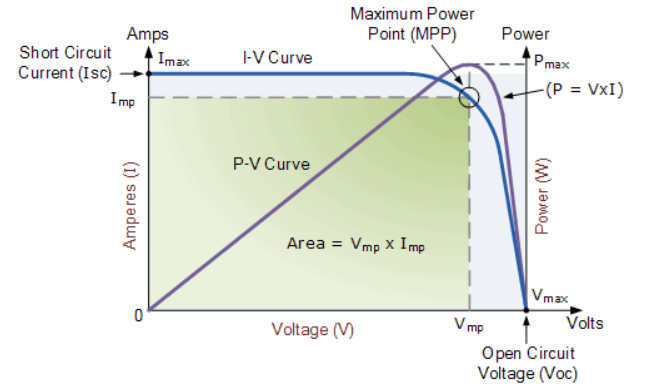
\includegraphics[width=0.88\linewidth]{../Pictures/IVcurve}
		\caption{I-V characteristics of a generic solar panel \cite{IVcurves}.}
		\label{fig:mpp}
	\end{center}
\end{figure}

From the P-V curve, the maximum power generated by the solar panel ($P_{max}$) is obtained. This maximum power corresponds to the MPP and takes place for a specific combination of voltage ($V_{mpp}$) and current ($I_{mpp}$). Therefore, the ideal operating point of a PV panel corresponds to the MPP which varies according to the level of solar radiation and the temperature \cite{handbook}. 

\newpage
There are different types of photovoltaic systems, however, the most common PV systems implemented nowadays are grid-connected \cite{handbook}. This type of PV system is mainly composed of a solar array, a DC-DC converter with an MPPT controller unit and an inverter, as shown in Figure \ref{fig:PVsystemblocks}. 

\begin{figure}[htbp]
	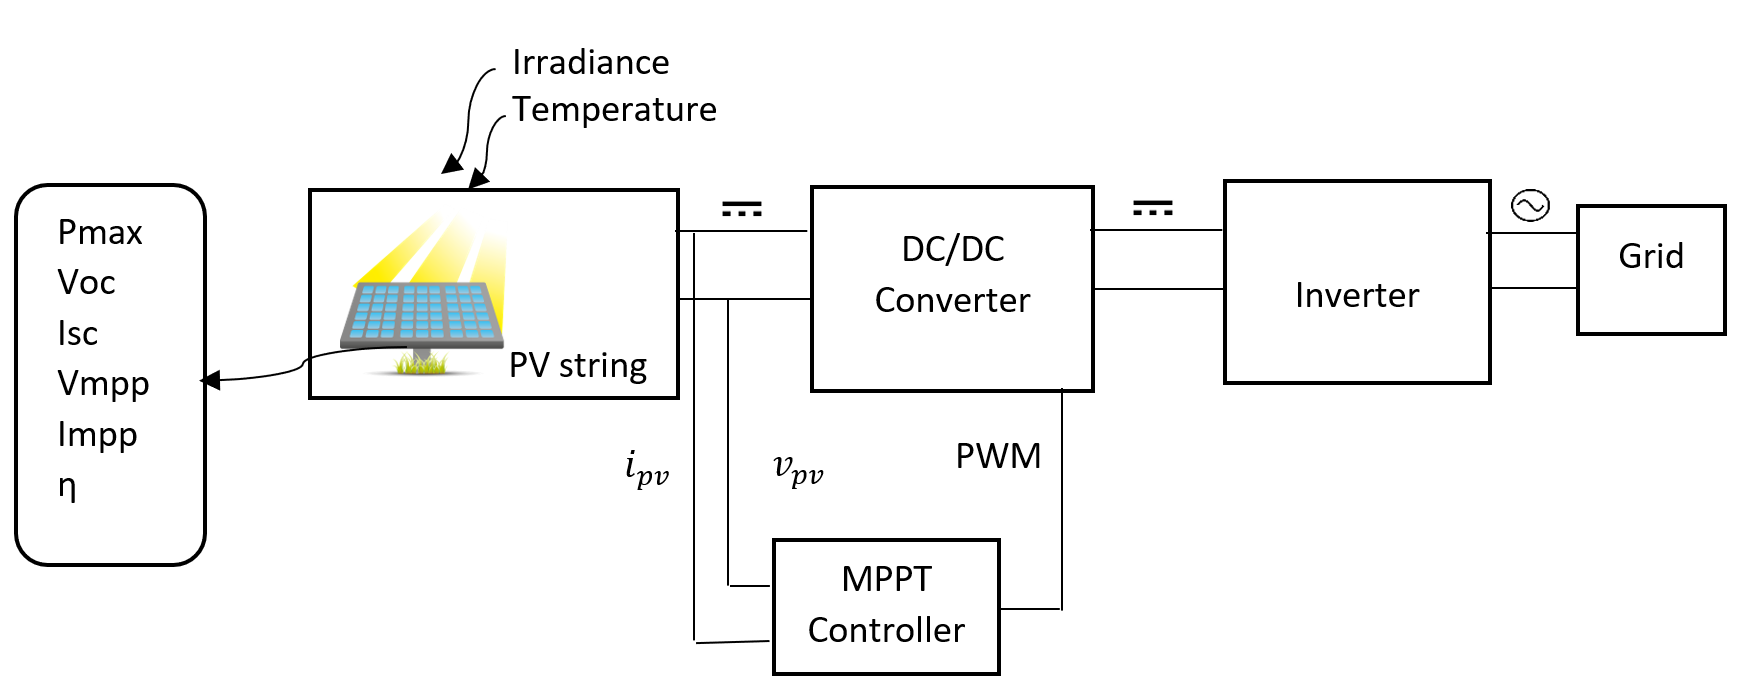
\includegraphics[width=\linewidth]{../Pictures/PV_system_blocks}
	\caption{Basic block diagram of a PV system.}
	\label{fig:PVsystemblocks}
\end{figure}

As mentioned at the begining of the chapter, PV modules can be connected to each other resulting in a PV array/string which generates electrical energy in the form of direct current. The MPPT controller unit takes the PV array's output voltage and current as input variables in order to calculate the ideal duty cycle. This duty cycle is used to vary the Pulse Width Modulation (PWM) signal of the DC-DC converter in order to get the PV string to work continuously at its MPP. The output of the DC-DC converter is connected to an inverter to convert the DC electric energy in an AC electrical signal compatible with the grid. 

 %PV systems can be classified in three main types: off-grid, grid-connection and grid-connection with battery backup (hybrid) systems \cite{handbook}. Off-grid systems are not connected to the grid which means that the power generated by the PV modules is stored in a battery bank for later use. In grid-tie systems the DC current is converted, using an inverter, into an AC current compatible with the grid. Nowadays, grid-tie systems are the most common, however, their main disadvantage is that they do not have battery backup. Which means that if there is a power outage the PV system will also be cut.  The solution to this problem is the grid-hybrid system which is a combination of a grid-tie system with a bank of batteries. This way it is possible to store energy and there is a battery backup in case of power outage. %[http://www.sabz-energy.com/solar%20electricity%20handbook%202017.pdf]
